\documentclass[a4paper]{article}

%%%%%%%% CREATE DOCUMENT STRUCTURE %%%%%%%%
%% Language and font encodings
\usepackage[english]{babel}
\usepackage[utf8x]{inputenc}
\usepackage[T1]{fontenc}
\usepackage{lmodern,textcomp}
%\usepackage{subfig}

\usepackage{pdflscape}

% code listings
\usepackage{listings}
\usepackage{xcolor}

\definecolor{codegreen}{rgb}{0,0.6,0}
\definecolor{codegray}{rgb}{0.5,0.5,0.5}
\definecolor{codepurple}{rgb}{0.58,0,0.82}
\definecolor{backcolour}{rgb}{0.95,0.95,0.92}

\lstdefinestyle{mystyle}{
    backgroundcolor=\color{backcolour},   
    commentstyle=\color{codegreen},
    keywordstyle=\color{magenta},
    numberstyle=\tiny\color{codegray},
    stringstyle=\color{codepurple},
    basicstyle=\ttfamily\footnotesize,
    breakatwhitespace=false,         
    breaklines=true,                 
    captionpos=b,                    
    keepspaces=true,                 
    numbers=left,                    
    numbersep=5pt,                  
    showspaces=false,                
    showstringspaces=false,
    showtabs=false,                  
    tabsize=2
}

\lstset{style=mystyle}

%% Sets page size and margins
\usepackage[a4paper,top=3cm,bottom=2cm,left=2cm,right=2cm,marginparwidth=1.75cm]{geometry}

%% Useful packages
\usepackage{pdfpages}
\usepackage{amsmath}
\usepackage{graphicx}
\usepackage[colorinlistoftodos]{todonotes}
\usepackage[colorlinks=true, allcolors=blue]{hyperref}
\usepackage{caption}
\usepackage{subcaption}
\usepackage{sectsty}
\usepackage{apacite}
\usepackage{float}
\usepackage{titling} 
\usepackage{blindtext}
\usepackage[square,sort,comma,numbers]{natbib}
\usepackage[colorinlistoftodos]{todonotes}
\usepackage{xcolor}
\definecolor{darkgreen}{rgb}{0.0, 0.4, 0.0}

\usepackage{lipsum}

%% Gantt chart package
\usepackage{pgfgantt}

%% Start sections on new pages
\usepackage{titlesec}
\newcommand{\sectionbreak}{\clearpage}

%% Wrap figures
\usepackage{wrapfig}

%%%%%%%% DOCUMENT %%%%%%%%
\begin{document}

%%%% Title Page
\begin{titlepage}

\newcommand{\HRule}{\rule{\linewidth}{0.5mm}} 							% horizontal line and its thickness
\center 
 
% University
\textsc{\LARGE The Hague University of Applied Sciences}\\[1cm]

% Document info
\textsc{\Large Image acquisition and processing}\\[0.2cm]
\textsc{\large Lab}\\[1cm] 										% Course Code
\HRule \\[0.8cm]
{ \huge \bfseries Final Report}\\[0.7cm]								% Assignment
\HRule \\[2cm]
\large
\emph{Author/Student:}\\
Luca van Straaten (18073611)\\													% Author info
Roderik Leijssen (15060292)\\[1.5cm]
\emph{Instructor:}\\
F.  Theinert\\[1.5cm]										
{\large \today}\\[5cm]
\includegraphics[width=0.6\textwidth]{images/hhs.png}\\[1cm] 	% University logo
\vfill
%update the version of document each time its modified after review
Document version 2.0
\end{titlepage}


\newpage
  \pagenumbering{roman}
  \tableofcontents
\newpage
\pagenumbering{arabic}

%%\begin{abstract}
%%Your abstract.
%%\end{abstract}

\graphicspath{ {./images/} }
\renewcommand{\thesubsection}{\thesection.\alph{subsection}}

%%%% SECTIONS
\setcounter{section}{-1}
\input{content/Introduction}
\input{content/Assignment_1}
\section {Assignment 2 \\ {Object in front of Dark Background}}
\label {sec:assignment_2}

For this assignment, we will be capturing a image wich we will also use for assignment 3 and 4. It will be of a model car in front of a dark background. 
The goal is to make a useful setup to acquire the image and solely adjust the exposuretime to come to a well exposed image \cite{Lab_Assignments}.

The code in Listing \ref{lst:expose_time_image} was used to take the image, or adjust the exposure time. The image was then saved in the folder from wich the program was run. for the full code see appendix \ref{sec:appendix_A}.

\begin{lstlisting}[language=C, caption=save image to file, label=lst:expose_time_image]
    case ' ':
        if (imgSave(image, "output.png")) {
            cout << "Image saved succesfully!" << endl;
        } else {
            cout << "Error saving file." << endl;
        }
        break;
        case ',':
        cam0.setExpoMs(--cfg.exposureMS);
        cout << "Exposure adjusted to " << cfg.exposureMS << endl;
        break;
        case '.':
        cam0.setExpoMs(++cfg.exposureMS);
        cout << "Exposure adjusted to " << cfg.exposureMS << endl;
        break;
        case '[':
        cam0.setExpoMs(cfg.exposureMS -= 10);
        cout << "Exposure adjusted to " << cfg.exposureMS << endl;
        break;
        case ']':
        cam0.setExpoMs(cfg.exposureMS += 10);
        cout << "Exposure adjusted to " << cfg.exposureMS << endl;
        break;
\end{lstlisting}

\subsection{Object with dark background}

\begin{figure}[h!]
    \centering
    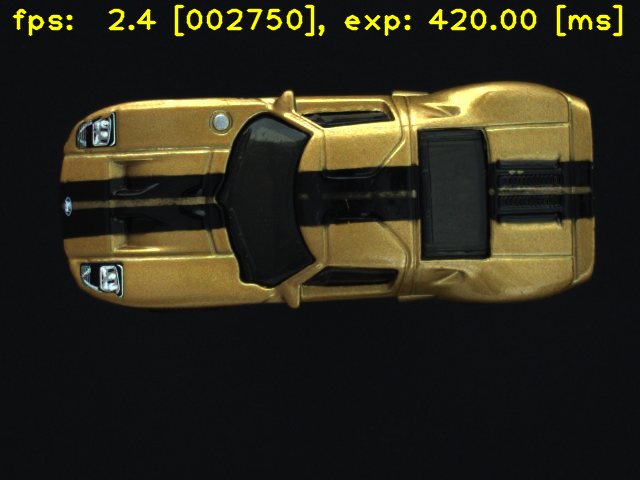
\includegraphics[width=0.45\textwidth]{ford_gt_final2.png}
    \caption{Object in front of Dark Background}
    \label{fig:fortgt}
\end{figure}

The image above is the image we took of the model car, it has a matelic gold paint with black stripes across. It was challenging to get the car well exposed, because the metallic paint is reflective. So we needed even light positioned in a way that the reflections would not go into the camera. Enough light was needed for the black parts of the car to not be ender exposed. We placed the object away from the background so we could make shine the light only on the car and not the background. The layout of the setup is shown in section \ref{sec:sketch}.

\subsection{Optimal exposure}

We got the best result using a 420 ms exposure time. This is the time the camera takes to gather light on the sensor. The image is shown in figure \ref{fig:fortgt}. The image is well exposed and the background is dark. The car is well visible and the details are clear. The image is not overexposed and the background is black but not saturated. 

\subsection{Sketch of setup}
\label{sec:sketch}

\begin{figure}[H]
    \centering
    \includegraphics[width=0.5\textwidth]{Lab_2_Diagram.png}
    \caption{Sketch of setup}
    \label{fig:sketch}
\end{figure}

\subsection{Calculation of ‘angle of view’}
\label{sec:angle_of_view}

% \begin{figure}[h!]
%     \centering
%     \includegraphics[width=0.35\textwidth]{ford_gt_final2_dimensies.png}
%     \caption{Angle of view reference image}
%     \label{fig:angleofview}
% \end{figure}

% The (horisontal) angle of view is the angle between the left and right part of the frame, and the camera lens. In order to calculate this we took a picture of a measuring tape stretching the full width of the frame at a known distance, 250 mm. See figure \ref{fig:angleofview} for this image. Now we calculate the angle of view:

% $$ \text{framewidth} = 90\text{mm} $$
% $$ \text{distance} = 250\text{mm}$$

% \begin{equation}
%     \theta = 2 \cdot \arctan{\frac{{\frac{\text{framewidth}}{2}}}{\text{distance}}} = 2 \cdot \arctan{\frac{\frac{90}{2}}{250}} = 2 \cdot \arctan{\frac{45}{250}} = 2 \cdot 19.8 = 39.6 \text{ degrees}
% \end{equation}

To calculate the angle of view $ \alpha $ we need the following information:

\begin{itemize}
    \item Sensor size [mm] $ d = 8.89 mm $
    \item focal length $ f = 6 mm $
\end{itemize}

And we used the following formula:

$$ \alpha = \frac{180}{\pi} \cdot 2\arctan{\frac{d}{2 \cdot f}} = \frac{180}{\pi} \cdot 2\arctan{\frac{8.89}{2 \cdot 6}} = 73.1 \text{ degrees} $$

\section {Assignment 3 \\ {Moving Object}}
\label {sec:assignment_3}

The description of this assignment was: Take an image of a considerably fast moving object (rotating disk) without any motion-blur and without reflection from any light-sources. You will not be able to synchronize the camera, so find a solution which will not need any synchronization.
Make a sketch of the required setup first, discuss multiple solutions in the group. \cite{Lab_Assignments}

\begin{lstlisting}[language=C, caption=save image to file, label=lst:50loop]
// capture 50 frames
if (capt50 == true) {
    capt50 = false;
    for(int i = 0; i < 50; i++) {
        cam0.captureFrame(&image);
        // save image with frame number
        imwrite("../capt/img" + to_string(i) + ".png", image);
    }
}
\end{lstlisting}


\subsection{Optimal exposure}

We use a strobe light to expose this image. The stroke frequency is not important but should be sufficiently slow to make it impossible for two exposures to occur in a single frame, and it should also be slow so that the capacitors inside the strobe enough time to charge to give the lights its maximum brightness. We took 50 images, and saved them to the file system. The first image which looks like \ref{fig:img36} was handpicked and the other images ware ignored. The image is slightly underexposed which could have been resolved with a lower RPM setting of the strobe, or by placing the strobe closer to the disc. Adding a difuser would eliminate reflections.

\begin{figure}[h!]
    \centering
    \includegraphics[width=0.35\textwidth]{img36.png}
    \caption{Image of moving object}
    \label{fig:img36}
\end{figure}

\subsection{Sketch of setup}

\begin{figure}[h!]
    \centering
    \includegraphics[width=0.65\textwidth]{Lab_3_Diagram.png}
    \caption{Sketch of setup}
    \label{fig:Lab_3_Diagram}
\end{figure}

\subsection{Calculation of ‘angle of view’}

We use the same camera and lens as assignment two, So the angle of view will be identical as calculated in section \ref{sec:angle_of_view}.

\section {Assignment 4 \\ {Salt and Pepper Noise}}
\label {sec:assignment_4}

\subsection{Manipulate own image from assignment 2}

In this assignment, a program was used to darken the image and add RGB salt and pepper noise to our original image from assignment 2. The noise must be filtered out and the brightness must be corrected.

We implemented a median filter and a gamma correction function to filter our image. The result is shown in figure \ref{fig:fortGT_Noise}.

\begin{figure}[h!]
    \centering
    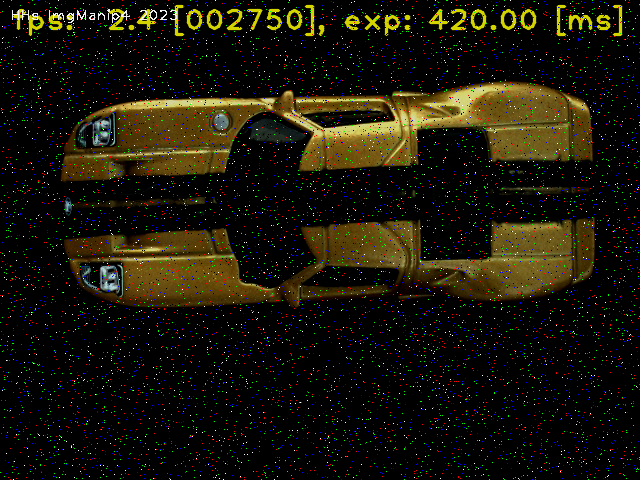
\includegraphics[width=0.45\textwidth]{fortGT_Noise.png}
    \caption{Image with salt and pepper noise}
    \label{fig:fortGT_Noise}
\end{figure}

\subsection{Write C/C++ code for Brightness correction}

A Brightness correction filter was written and can be found in appendix \ref{sec:appendix_B}. The filter function is shown in listing \ref{lst:brightness_correction}.

\begin{lstlisting}[language=C, caption={Brightness correction}, label=lst:brightness_correction]

void gammaCorrection(Mat* input, Mat* output, float gamma) {
    Size s = input->size();
    long h, w;
    float sum;
    
    std::cout << "Correcting gamma" << std::endl;
    uint8_t out[s.height][s.width];
    uint8_t lut[256];	
    
    for (int i = 0; i < 256; i++) { //create a lookup table, with the gamma correction curve.
        lut[i] = saturate_cast<uint8_t>(pow((float)(i / 255.0), gamma) * 255.0f); //saturate cast negative values to 0, and higher values to 255 (uint8_t or unsigned char)
        //std::cout << unsigned(lut[i]) << " "; //print the function for testing. cout prints uint8_t as chars so we cast it.
    }
    
    
    for (w=0; w<s.width; w++){ //loop over the image, 
        for(h=0; h<s.height; h++){
            sum = lut[(input->at<uint8_t>(h,w))]; //the original output value will be scaled to the value in the LUT.
            out[h][w]=(uint8_t)sum;
        }
    }
    std::memcpy(output->data, out, s.height*s.width*sizeof(uint8_t)); //copy our standard 2D array to a new buffer that OpenCV understands
}

We had several options for correcting brightness. At first we considered simply increasing the value of each pixel by addition. However, this would significantly increase the brightness of the black background turning it dark grey. For this reason we settled on using a gamma correction curve instead. This would spread the histogram "bins" rather than moving them up. Determining the correct gamma correction constant was trial and error, exponents below 0,5 would make the object too bright. 

\end{lstlisting}

\subsection{Write C/C++ code for ‘Salt and Pepper Noise’ correction}

A ‘Salt and Pepper Noise’ correction filter was written and can be found in appendix \ref{sec:appendix_B}. The filter function is shown in listing \ref{lst:noise_filter}.

\begin{lstlisting}[language=C, caption=Noise correction filter, label=lst:noise_filter]
void filter(Mat* input, Mat* result) {
    Size s = input->size();
    long h, w;
    long sum;
    
    //std::cout << "Input type was : " << input->type() << std::endl;
    uint8_t out[s.height][s.width];
    
    std::cout << s.height << " " << s.width << std::endl;
    
    for (w=0; w<s.width; w++){ //loop over the image, 
        for(h=0; h<s.height; h++){
            sum = 0;
            std::vector<uint8_t> median;
            
            for (int _x = -1; _x < 2; ++_x) //for every pixel, loop over every pixel in a 3x3 kernel
            {
                for (int _y = -1; _y < 2; ++_y)
                {
                    int idx_y = h + _y; //sum the incrementor with the kernel's, so we can identify borders
                    int idx_x = w + _x;
                    
                    if (idx_x < 0 || idx_x > s.width) //the kernel goes outside of the image, therefore break and ignore that pixel.
                        break;
                        
                    if (idx_y < 0 || idx_y > s.height)
                        break;
                    
                    median.push_back(input->at<uint8_t>(idx_y,idx_x)); // Add all the pixels from the kernel into a vector
                }
            }
            std::sort(std::begin(median), std::end(median)); //sort all pixel values from high to low
                    
            for (auto it = median.begin(); it != median.end(); ++it) {
                sum = median.at(median.size()/2); //The pixel at the y,x coordinate is now the median from our 3x3 sliding window
            }
            out[h][w]=(uint8_t)sum;
        }
    }
    // this did not work, since the out array was never copied to memory, causing image data pointing to nowhere!
    //result = Mat(s.height, s.width, CV_8U, out); 
    // Instead, the data from out needs to be copied directly to Mat result with the correct size
    std::memcpy(result->data, out, s.height*s.width*sizeof(uint8_t));
}

The reason why we chose to implement a median filter is to preserve sharp edges to minimize loss of detail on the object, whereas a Gaussian or mean filter would blur sharp edges. In our code, a 3x3 sliding window is ran over the image, and the center pixel is replaced with the median of the window. The pixel values from the kernel are pushed back into a std::vector, this allows us to use STL library operations like std::sort to order the values.
After applying the median filter, the resulting image looks slightly blurred, but sharp transitions are mostly preserved. Note that the 1px wide text at the top of the image is partially removed. This is due to the nature of a median filter and is very challanging to preserve.

\end{lstlisting}

The result after applying the noise removal filter is snow below \ref{fig:fortGT_Noise_Filtered}.
\begin{figure}[h!]
    \centering
    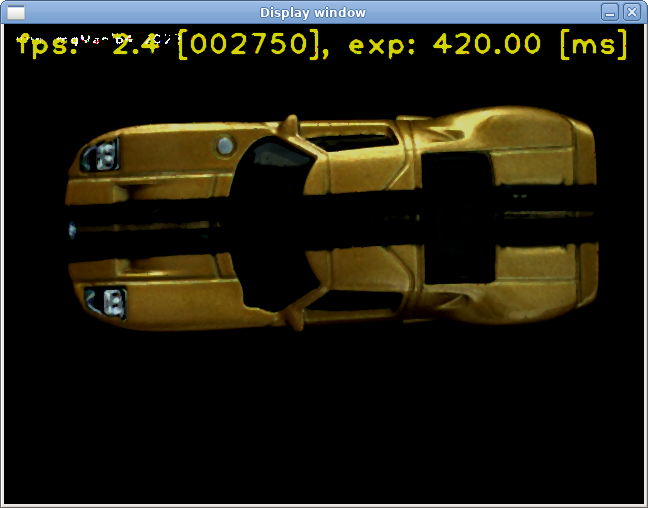
\includegraphics[width=0.45\textwidth]{fortGT_Noise_Filtered.png}
    \caption{Filtered image}
    \label{fig:fortGT_Noise_Filtered}
\end{figure}

The final result is shown in the figure below \ref{fig:fortGT_Filtered_corrected_05}. We chose a gamma correction factor of 0.5 but other values can also be used.
\begin{figure}[h!]
    \centering
    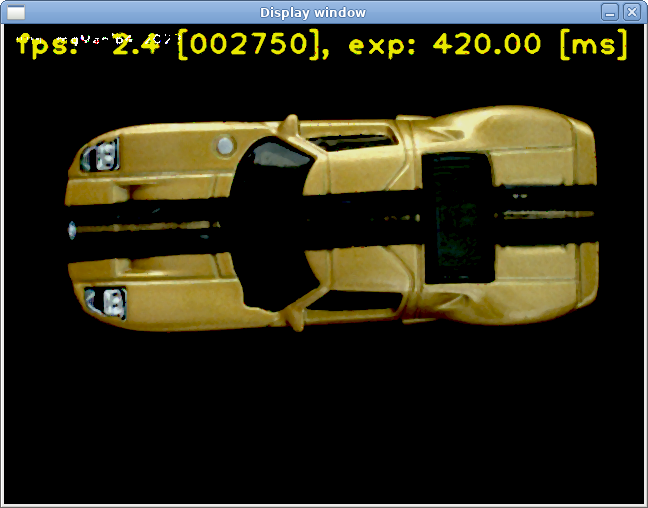
\includegraphics[width=0.45\textwidth]{fortGT_Filtered_corrected_05.png}
    \caption{Gamma correction on the filtered image}
    \label{fig:fortGT_Filtered_corrected_05}
\end{figure}

\section {Assignment 5 \\ {Convolution}}
\label {sec:assignment_5}

We wrote a convolutie 5x5 kernel with all 1's. The kernel put over the image from lab 2 is shown in figure \ref{fig:5x5}. Note how the output of the filter will slightly blur the image.

\begin{figure}[h!]
    \centering
    \includegraphics[width=0.45\textwidth]{5x5.png}
    \caption{5x5 kernel over image from lab 2}
    \label{fig:5x5}
\end{figure}

The code we used to make the kernel is shown in listing \ref{lst:5x5}. and the full code can be found in appendix \ref{sec:appendix_C}.

We slightly deviated from the original assignment function prototype by replacing the int* argument to a 2D array pointer. We think that is not possible to easily call the kernel by reference without changing this argument, and makes the function more sensible to use. The size is fixed at compile time however.

The code does not make use of any OpenCV iteration templates, which would have drastically improved the performance. However, the assignemnt stated that it was not allowed to rely on OpenCV functionality despite having to use the cv2::Mat class.

The code below will loop over the height and width of the image, and on each pixel loop through the kernel passed as an argument. The result is the use of nested for loops, which quadratically increases processing time. It is highly inefficient and took roughly 13 seconds to execute on my machine (5587.52 BogoMips)

\begin{lstlisting}[language=C, caption=5x5 kernel, label=lst:5x5]
    //int* from original assignment replaced with pointer to the kernel instead, because that makes more sense
    void convolve5 (Mat* inputImg, Mat* outImg, int (*kernel5)[5][5]) { 
        //I assume the mat is CV_8UC1 since I want to process BGR channels individually
        Size s = inputImg -> size(); // get size of image
        const uint8_t kernel_size = 5; // todo: replace with sizeof
        uint8_t out[s.height][s.width]; // create output array
        int x ,y, h, w, i, j, sum; // declare variables
        
        std::cout << "Input type was : " << inputImg->type() << std::endl; //debug
      
        for (h=0; h<s.height; h++) { // for each row
            for(w=0; w<s.width; w++){ // for each column
                sum = 0; // reset sum
                for(i=0 ;i<kernel_size; i++ ){ // for each kernel row
                    for(j=0; j<kernel_size; j++){ // for each kernel column
                        y=h-i+1; x=w-j+1; // calculate the position of the pixel in the image
                        // if the pixel is outside the image, set it to the border
                        if(y<0) y=0;
                        if(y>s.height-2) y=s.height-2; 
                        if(x<0) x=0;
                        if(x>s.width-2) x=s.width-2;
                        sum += ((*kernel5)[i][j]) * inputImg->at<uint8_t>(y,x); // add the product of the kernel and the pixel to the sum
                    }
                }
                sum /= kernel_size*kernel_size; //divide the result of the pixel by 5^2
                if(sum<0) sum=0; // if the result is negative, set it to 0
                if(sum>255) sum=255; // if the result is greater than 255, set it to 255
                std::memcpy(outImg->data, out, s.height*s.width*sizeof(uint8_t)); // copy the result to the output array
                out[h][w]=(uint8_t)sum; // set the result to the output array
            }
        }
    }
    
\end{lstlisting}

\section {Assignment 6 \\ {Demosaicing Filter}}
\label {sec:assignment_6}

\subsection{Write C/C++ code for capturing a raw image}

\begin{lstlisting}[language=C, caption=save image to file, label=lst:rawcode]
// capture raw image
imshow(camName, image);
if (captRAW == true) {
    captRAW = false;
    // save raw image
    cfg.camMode = CAM_MODE_RAW;
    cam0.captureFrame(&image);
    imwrite("../capt/RAW.png", image);

    // save color image
    cfg.camMode = CAM_MODE_COL;
    cam0.captureFrame(&image);
    imwrite("../capt/COL.png", image);
}
\end{lstlisting}

\subsection{Convert this grayscale image to a color image by implementing a function to recover the actual colors}
The function prototype should look as follows:
\begin{lstlisting}[language=C, caption=function prototype, label=lst:prototype]
void deBayer(Mat *rawImg, Mat *outImg);
\end{lstlisting}

% \section {Conclusion}
\label {sec:conclusion}



%%%%%%%% EXTRA TIPS %%%%%%%%
%% hou deze structuur aan voor afbeeldingen
%%\begin{figure}[H]
%%\includegraphics[]{Pendulum.jpg}
%%\caption{Sketch of the pendulum}
%%\label{fig:pendulum}
%%\end{figure}


\newpage
\bibliographystyle{apacite}
\bibliography{ref}

\newpage
\appendix
\section{Appendix A}
\label{sec:appendix_A}

\includepdf[pages=-]{./appendix/hhs_cam.cpp.pdf}

\section{Appendix B}
\label{sec:appendix_B}

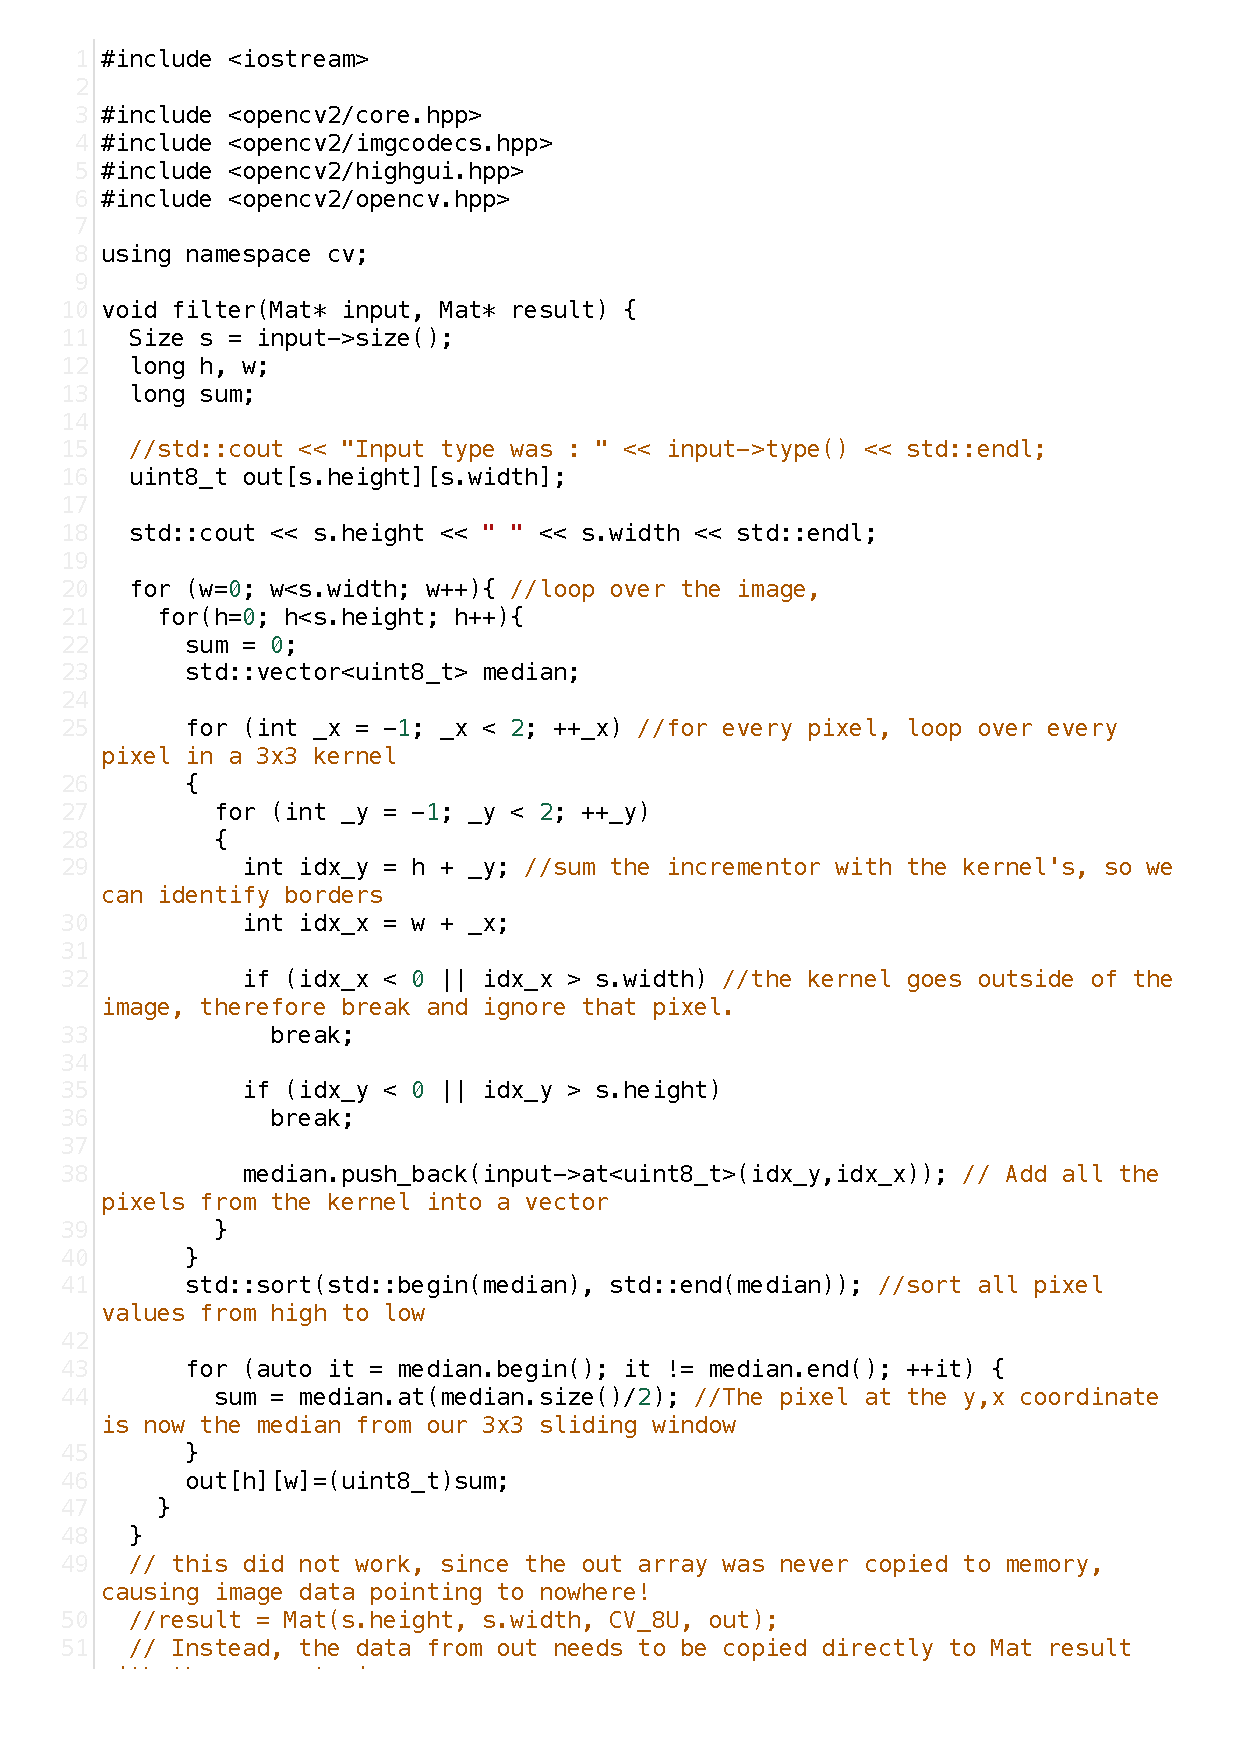
\includepdf[pages=-]{./appendix/main.cpp.pdf}

\section{Appendix C}
\label{sec:appendix_C}

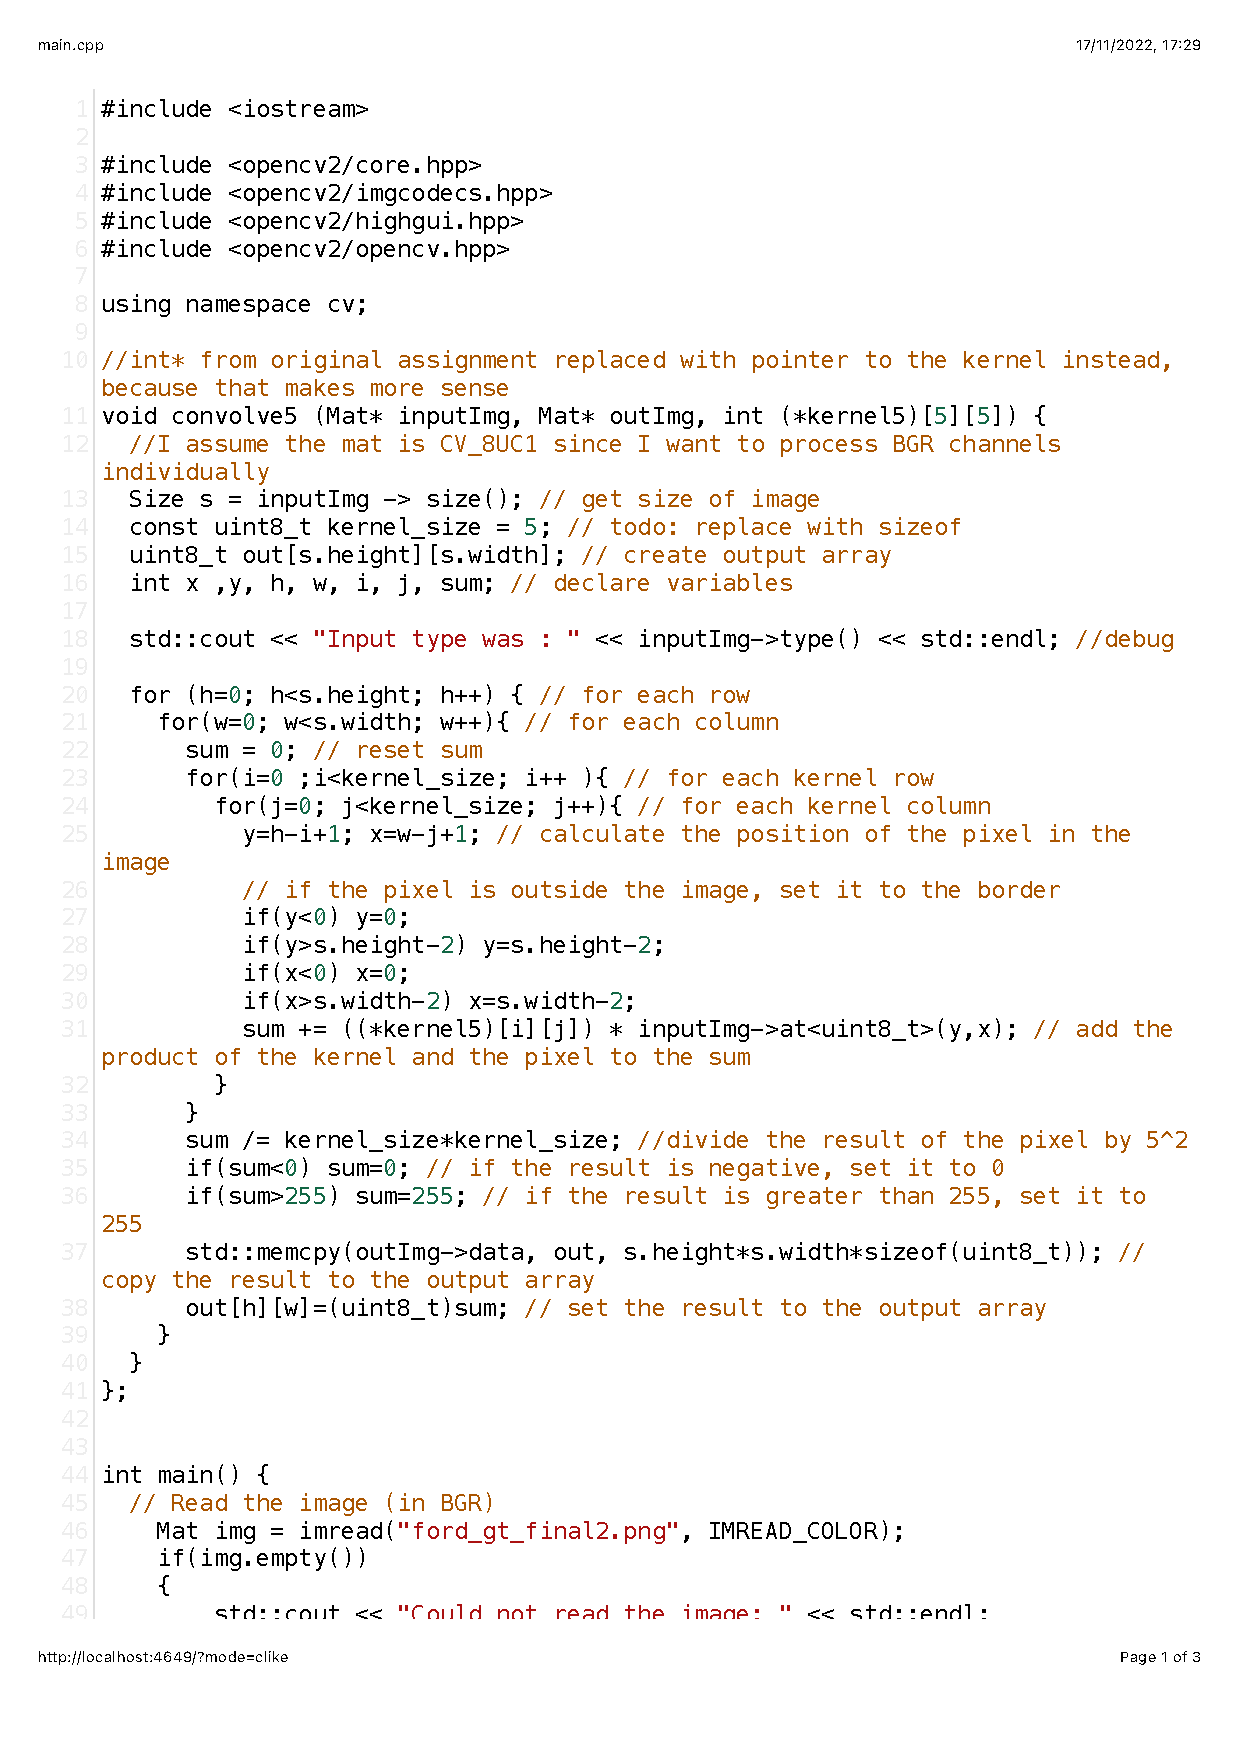
\includepdf[pages=-]{./appendix/5convilution.pdf}

\section{Appendix D}
\label{sec:appendix_D}

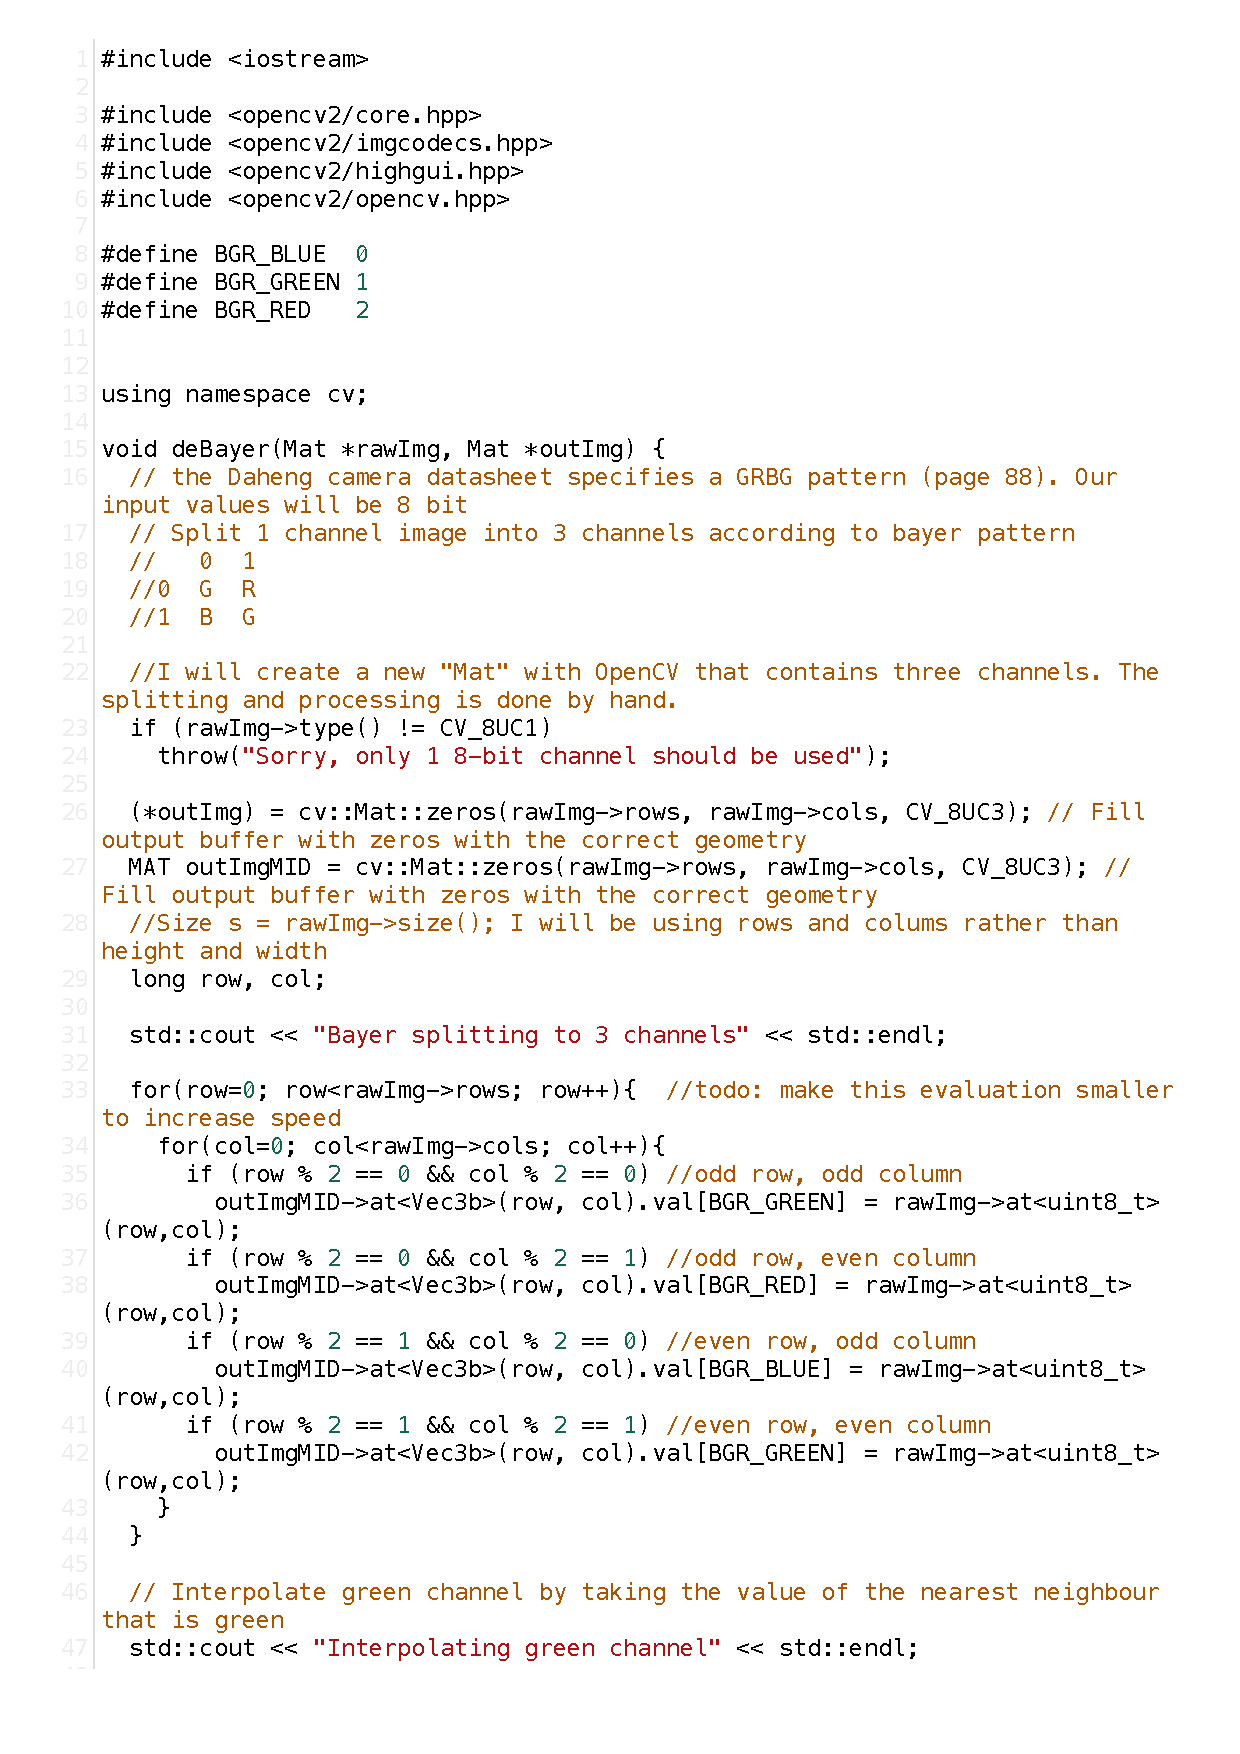
\includepdf[pages=-]{./appendix/6.pdf}

\end{document}